%
% Enkonduko speciala por Dua Libro
%

% Ni bezonas germanajn citaĵojn
% 
\usepackage{csquotes}
\MakeOuterQuote{"}
\setquotestyle{german}

% kalkuloj
%
\usepackage{calc}

%
% TIPAROJ
%

% ... el dafont
\newfontfamily\latino{MkLatinoPlain}[LetterSpace=20]

% titlesec -- pli bonaj titoloj por ĉapitroj kaj sekcioj
%
% memoru:
% titleformat{command}[shape]{format}{label}{sep}{before-code}[after-code]
%

\renewcommand{\thesection}{\arabic{section}}
\titleformat{\section}[display]{\centering\large\bf}{}{0pt}{\phantomsection\scalebox{2}[1]}
\titlespacing{\section}{0pt}{1em}{1em}
\titleformat{\chapter}[display]{\centering}{}{0pt}{\cowboyfont\Large}

\newcommand\mychap[1]{%
\chapter*{\protect\scalebox{2}[1]{\MakeUppercase{#1}}}
\addcontentsline{toc}{chapter}{#1}
}


\newcommand\mychapbig[1]{%
\phantomsection
\chapter*{\protect\scalebox{2}[1]{#1}}
\addcontentsline{toc}{chapter}{#1}
}

\newcommand\mysect[1]{%
\section*{#1}
\addcontentsline{toc}{section}{#1}
}

% Tiu desegnas la "kajero" skatolon sur la titolopaĝo
%
\newcommand{\kajerobox}{%
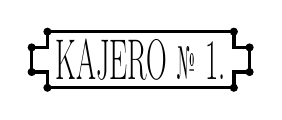
\begin{tikzpicture}[every node/.style={inner sep=0pt}]
\node[align=center](Text){\scalebox{0.5}[1]{\huge{\copper{KAJERO}} {\LARGE \textnumero} \copper 1.}};
\coordinate[shift={(-0.1cm,0.1cm)}](A) at (Text.north west);
\coordinate[shift={(0.1cm,0.1cm)}](B) at (Text.north east);
\coordinate[shift={(0.1cm,-0.1cm)}](C) at (Text.north east);
\coordinate[shift={(0.3cm,-0.1cm)}](D) at (Text.north east);
\coordinate[shift={(0.3cm,0.1cm)}](E) at (Text.south east);
\coordinate[shift={(0.1cm,0.1cm)}](F) at (Text.south east);
\coordinate[shift={(0.1cm,-0.1cm)}](G) at (Text.south east);
\coordinate[shift={(-0.1cm,-0.1cm)}](H) at (Text.south west);
\coordinate[shift={(-0.1cm,0.1cm)}](I) at (Text.south west);
\coordinate[shift={(-0.3cm,0.1cm)}](J) at (Text.south west);
\coordinate[shift={(-0.3cm,-0.1cm)}](K) at (Text.north west);
\coordinate[shift={(-0.1cm,-0.1cm)}](L) at (Text.north west);
\draw[very thick](A) -- (B) -- (C) -- (D) -- (E) -- (F) -- (G) -- (H) -- (I) -- (J) -- (K) -- (L) -- cycle;
\filldraw(A) circle [radius=1.25pt];
\filldraw(B) circle [radius=1.25pt];
\filldraw(D) circle [radius=1.25pt];
\filldraw(E) circle [radius=1.25pt];
\filldraw(G) circle [radius=1.25pt];
\filldraw(H) circle [radius=1.25pt];
\filldraw(J) circle [radius=1.25pt];
\filldraw(K) circle [radius=1.25pt];
\end{tikzpicture}}

% La komando por la intermorfema streko. 
% Ne la sama kiel la komando en Unua Libro
%
\renewcommand{\,}{\raisebox{-1.1ex}{\relsize{-0.5}{\textquotesingle}}}

% bufro por Nomaro
%
\newlength{\xxx}
\newcommand\buffer{\hspace*{3em}—\hspace*{3em}}
\settowidth{\xxx}{\buffer}
